\documentclass{report}

\input{preamble}
\input{macros}
\input{letterfonts}

\title{\Huge{AP Physics C}\\Equipotential Lab}
\author{\huge{Ben Feuer}}
% Wens, March 6th, 2024
\date{\huge{Wednesday, March 6th, 2024}}

\begin{document}

\maketitle
\newpage% or \cleardoublepage
% \pdfbookmark[<level>]{<title>}{<dest>}
\pdfbookmark[section]{\contentsname}{toc}
% \tableofcontents
% \pagebreak

\begin{figure}[h!]
  \begin{center}
    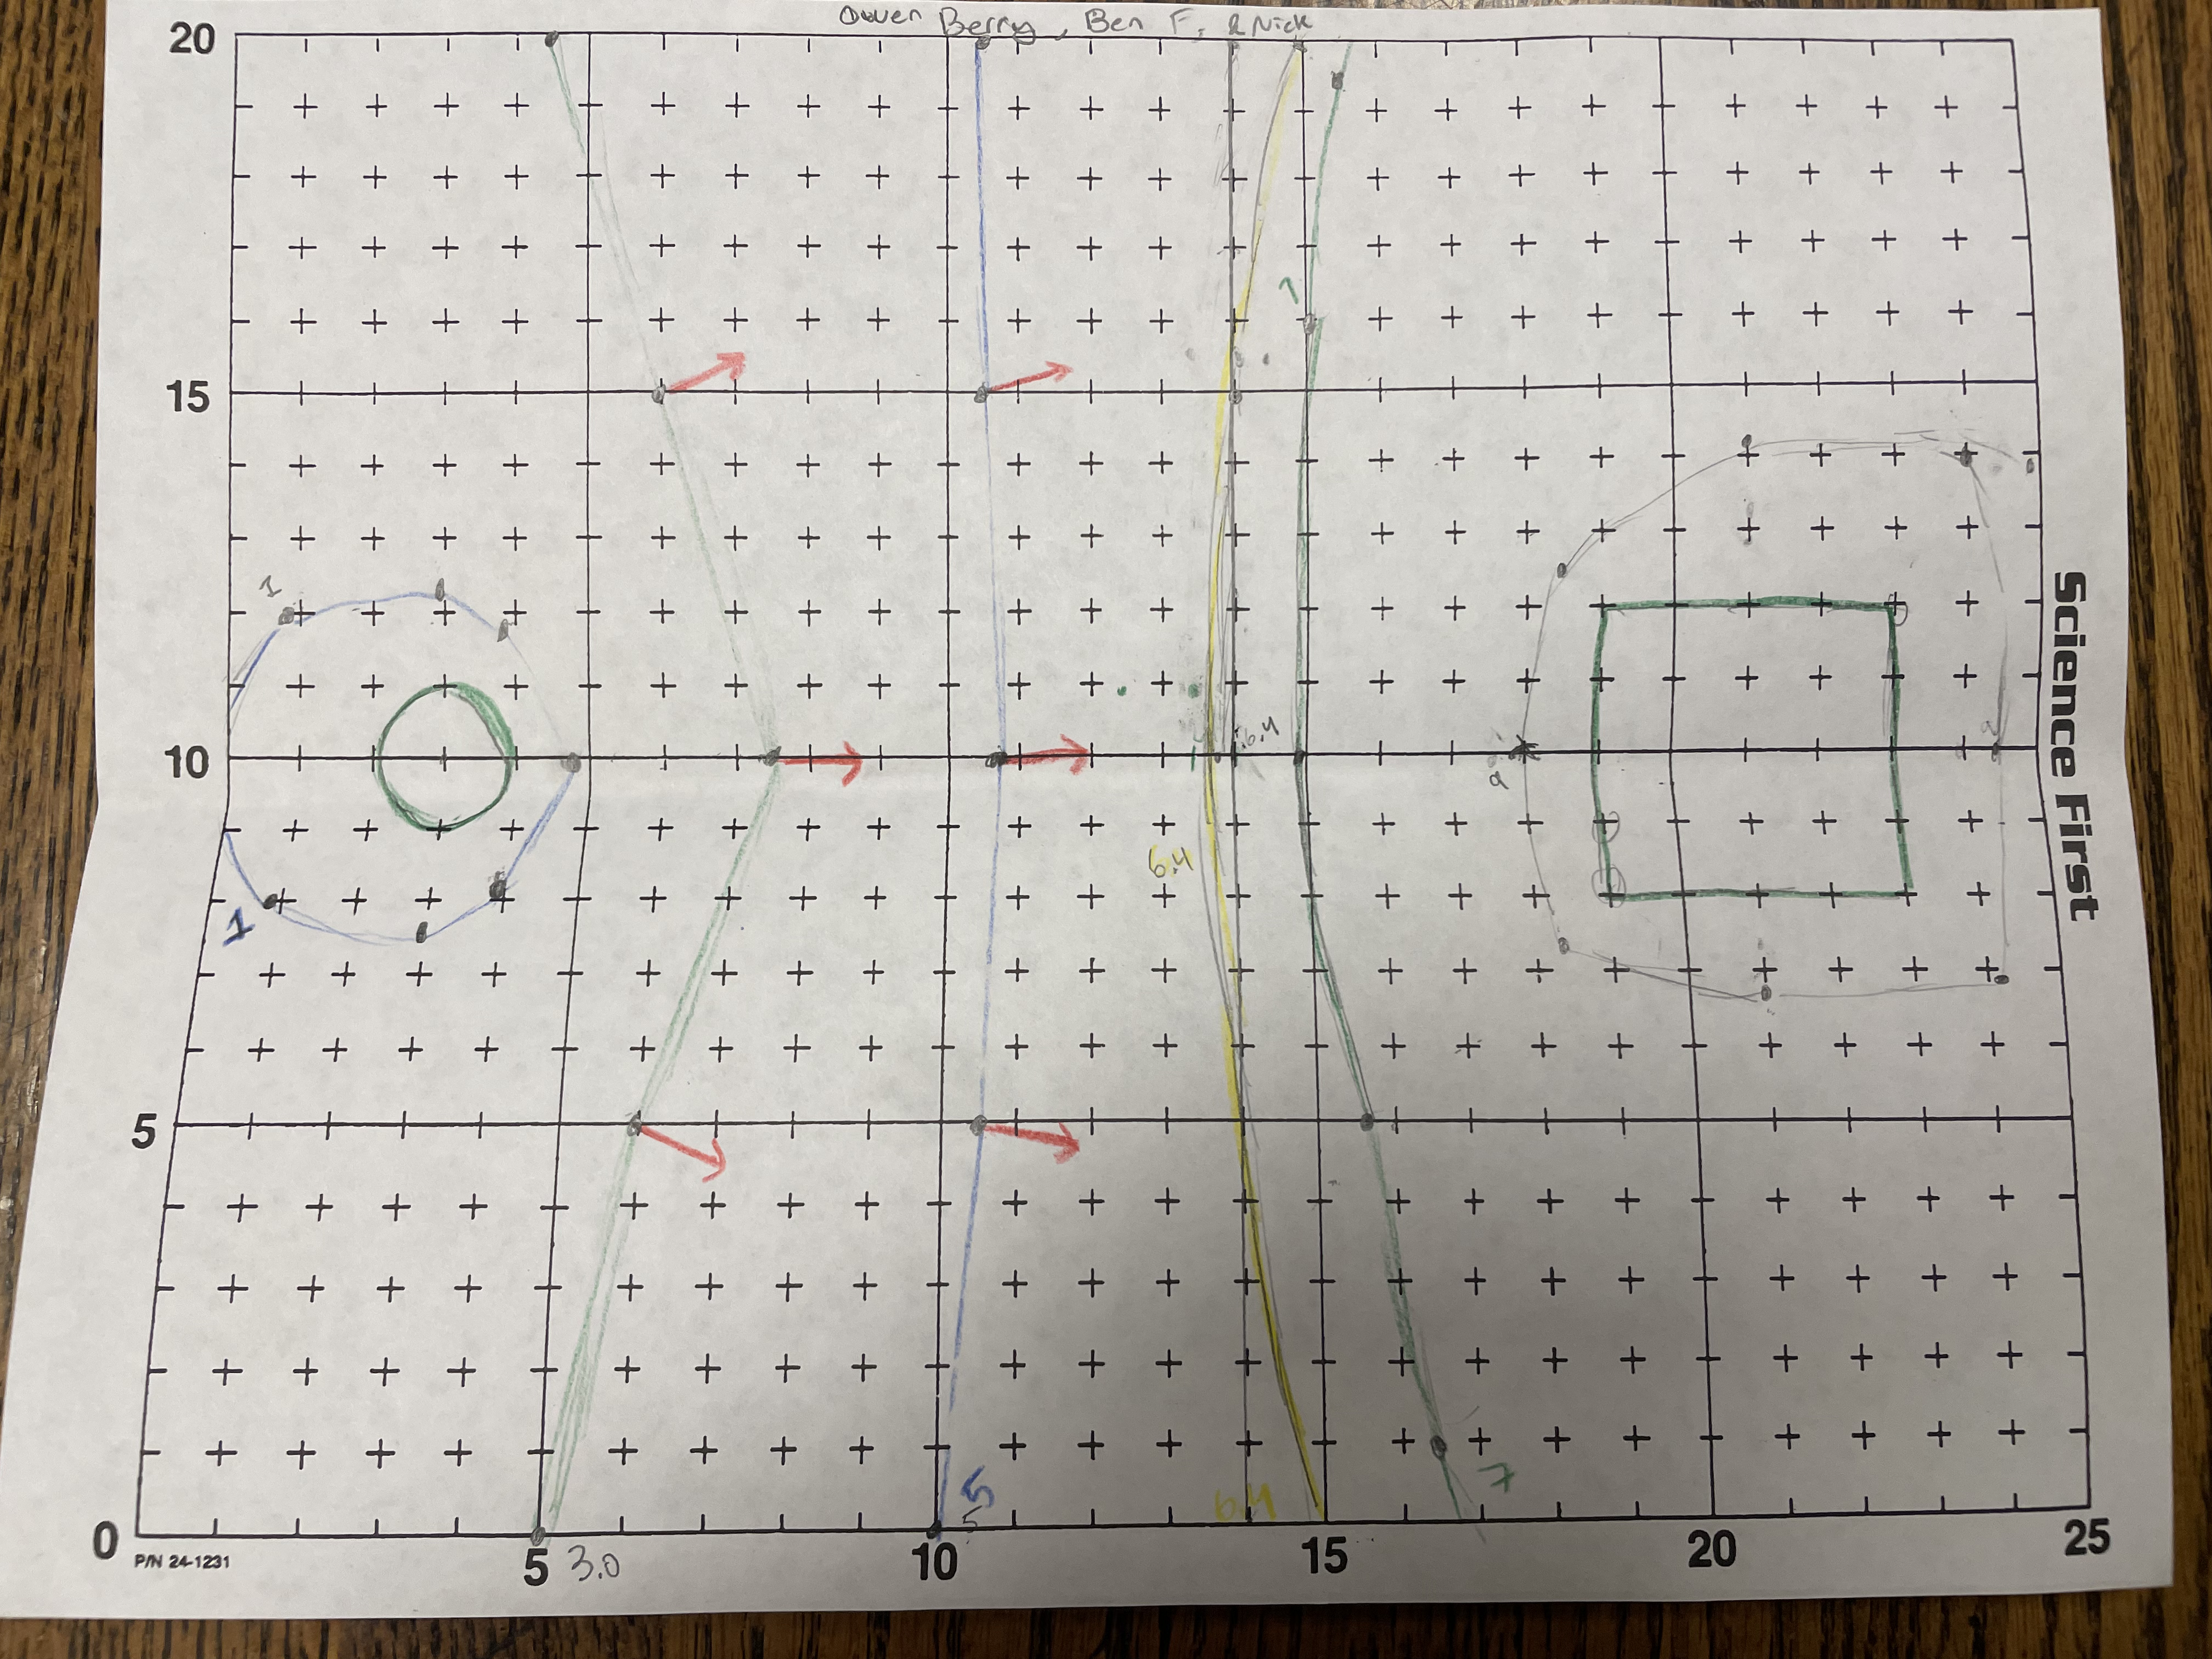
\includegraphics[width=0.95\textwidth]{figures/Equipotential.png}
  \end{center}
  \caption{Equipotential Sketch (note the elctric field should be pointing to the left, not right)}
\end{figure}

\qs{How much work would it take to move a $ 2\mu $ C charge from 3V to 7V? }{
  $$ W =  - \Delta U = -q \Delta V =  - (2\mu C)(7V - 3V) = 8\mu J = - 8 \times 10^{-6} J \text{ this is negative} $$
}

\qs{\small{Would a $-4\mu$ C starting on a 5V surface be more likely to move to a 7V or 3V surface?}}{
  Becuase the electric field shown on the sketch is pointing to the left(the sketch is wrong), which is where the 3V surface is, the $-4\mu$ C charge \textbf{would more likely to move to right, where the 7V surface is}, because the negative charge will have a force in the opposite direction of the electric field.
}

\qs{How much work would it take to move a proton along the 9V surface?}{
  It would take no work to move a proton along the 9V surface because the electric potential is constant along the 9V surface as it is an equipotential surface, and therefore \textbf{the work done is zero}.
}

\qs{An electron moves from the 1V surface to the 5V surface.}{
  \textbf{Did it gain or lose potential energy? How much?} \\
  $$ \Delta U = q \Delta V = (-1.6 \times 10^{-19}) (5V-1V) = - 6.4 \times 10^{-19} J \text{ loss of potential energy}$$  \\
  \textbf{Did it gain or lose kinetic energy? How much?} \\
  If energy is conserved, then there would be a gain of kinetic energy opposite to theloss of potential energy, which is equal to $ +6.4 \times 10^{-19} J $. \\
  \textbf{How would your answers to a and b change (if at all) if it was a proton moving between the same two points?
} \\
  If it was a proton, the charge would be positive meaning the change in potential energy would be $ + 6.4 \times 10^{-19} J $ instead of $ - 6.4 \times 10^{-19} J $. Change in kinetic energy likewise would then be $ - 6.4 \times 10^{-19} J $ instead of $ + 6.4 \times 10^{-19} J $
}

\qs{Potential and Electric Field for the "floating conductor"}{
  \textbf{a. Why did you need to record only a single value of potential for your "floating" (not connected to the electrodes) conductors?} \\
  Because the "floating conductor" is an area surrounded by a conductor, the electric field is equal to zero throughout the inside surface (similar to the elctric field inside a sphere with a conducting surface) and therefore there with no change in electric field throughout the surface, the potential is constant according to the equation: $ \Delta  V = \int E dx $. \\
  \textbf{b. What can you say about the electric field inside your "floating" conductors? Explain.} \\
  The electric field inside the "floating conductor" is zero as said in the prior question. This can be further explained under the fact that negative charges are equally distributed surrounding the "floating conductor" area applying oppositing force that cancel out.
}

\end{document}
